%!TEX root = ../../root.tex

Il data model è stato costruito usando il diagramma della classi UML, ed è diviso in due principali package: uno rappresenta la modellazione degli statement, il secondo rappresenta la modellazione dei vari modelli. Di seguito è mostrata l'immagine che rappresenta l'intero data model:
\begin{figure}[H]
	\centering
	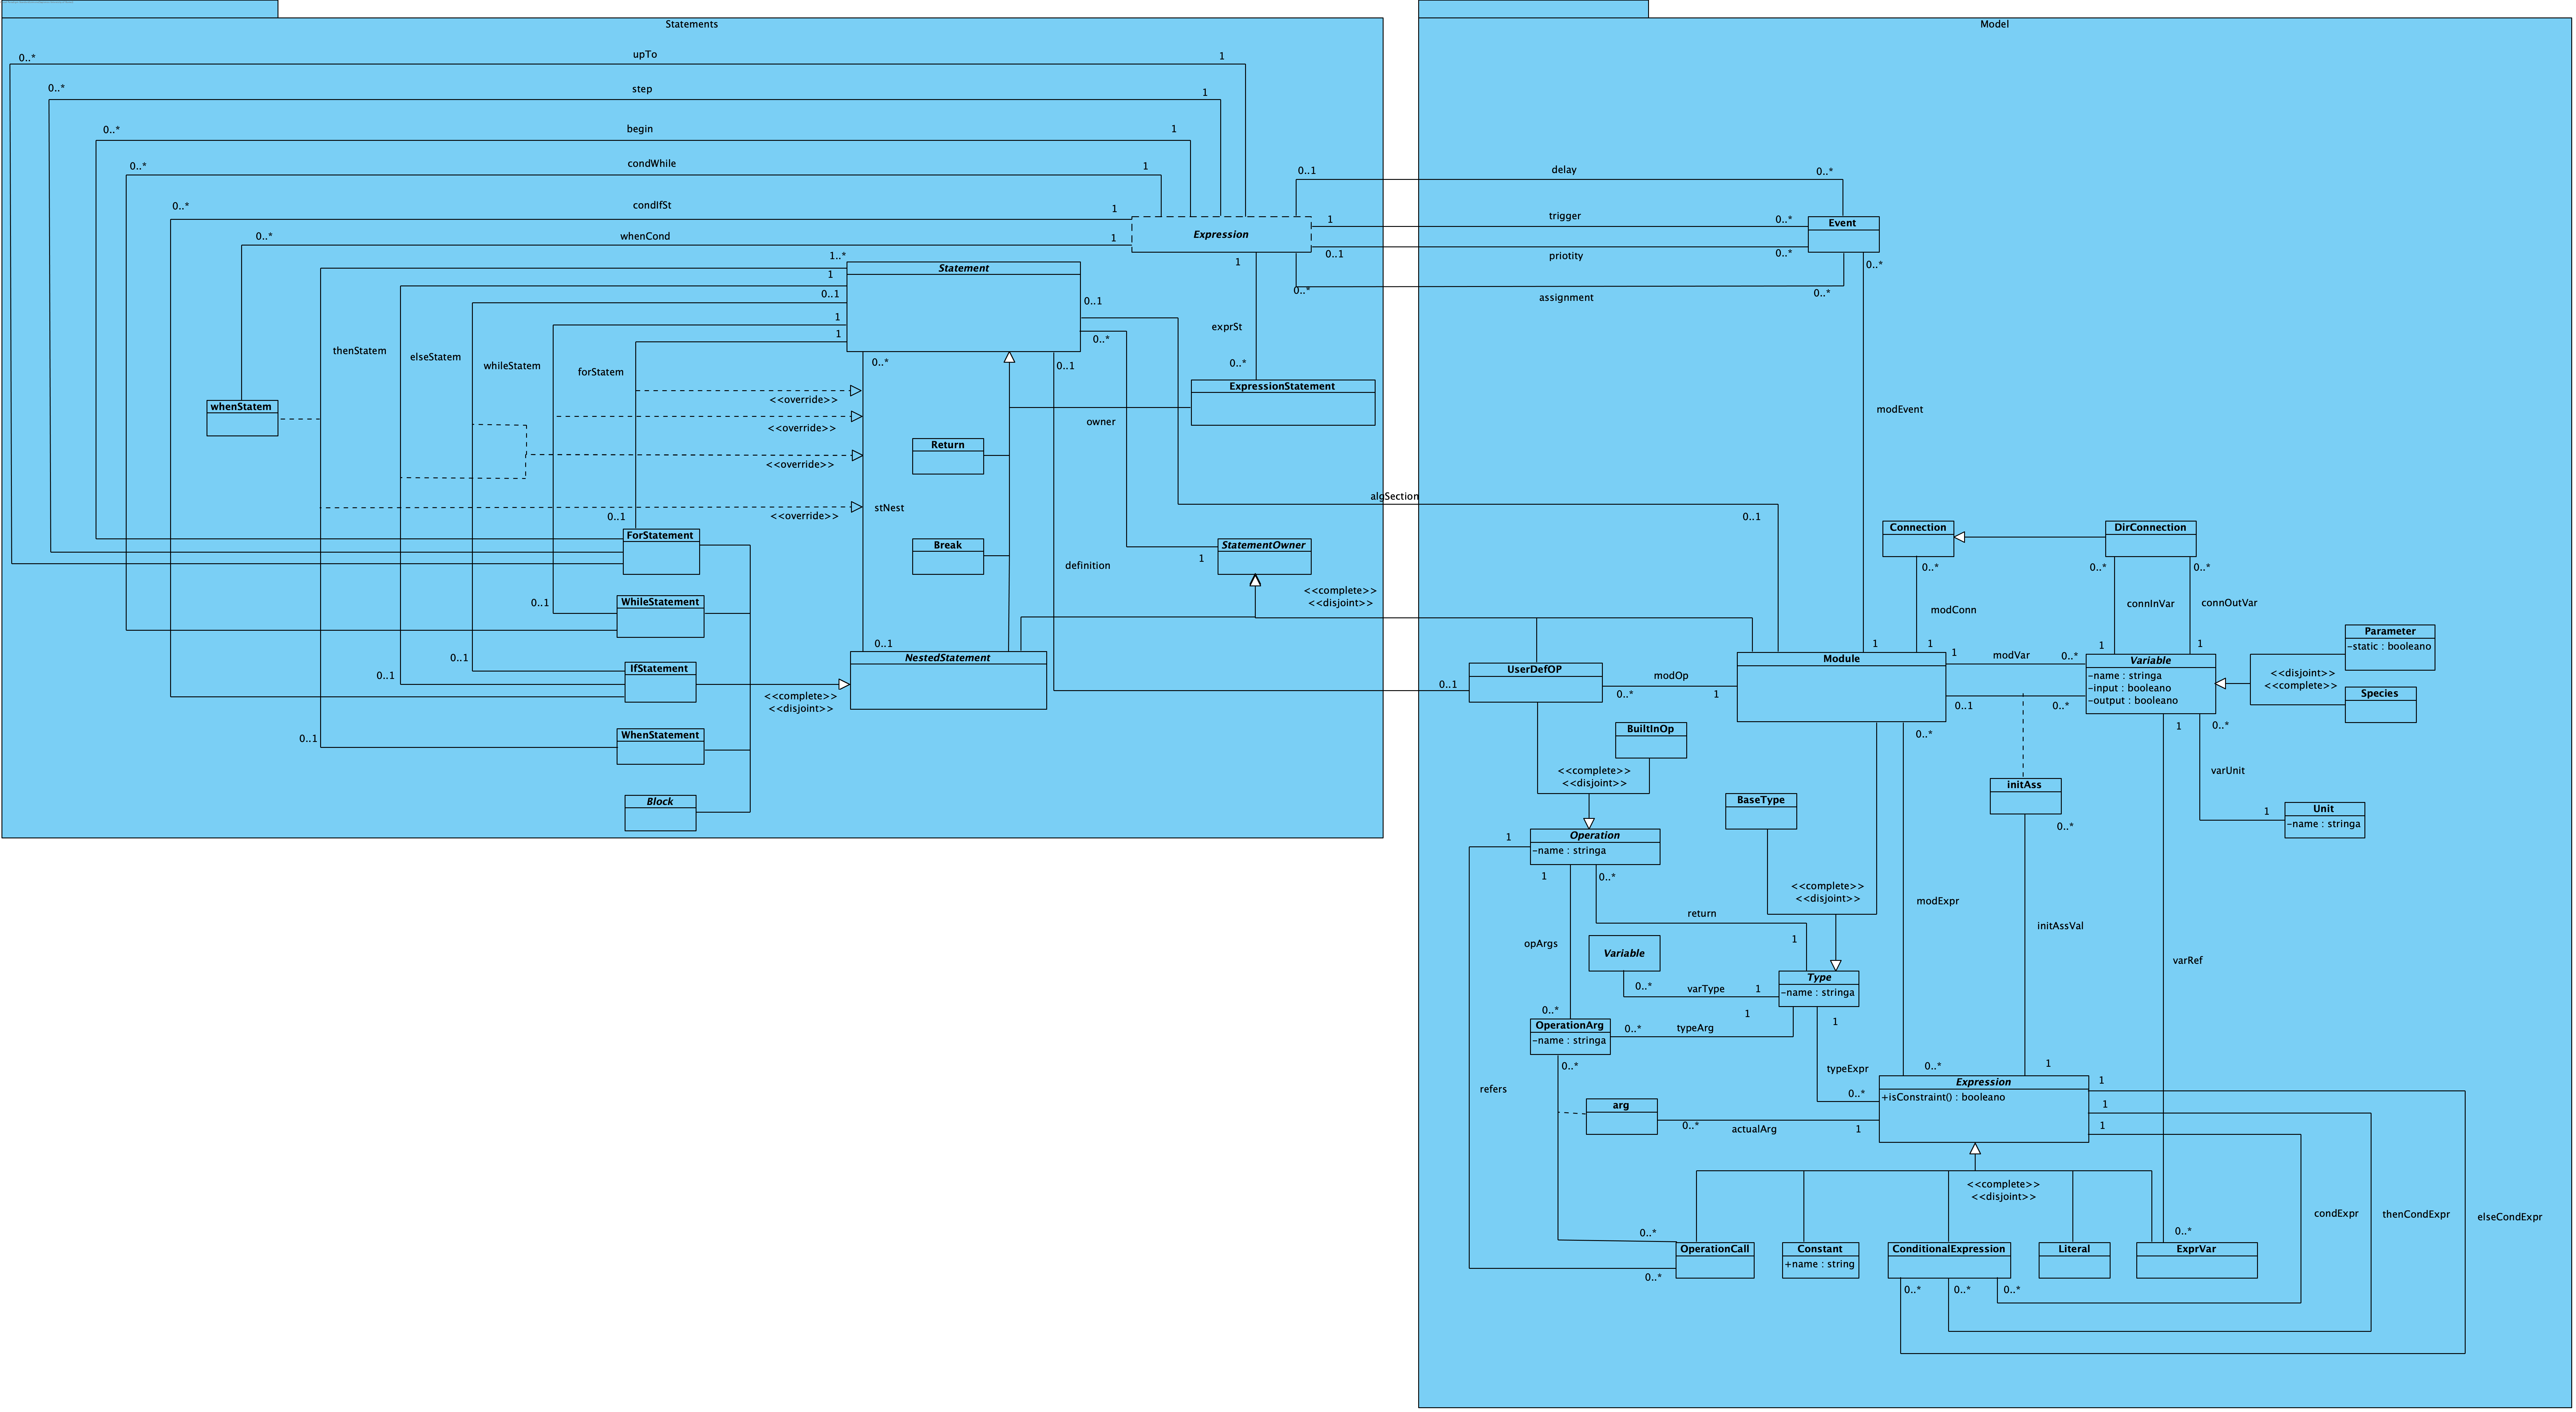
\includegraphics[width=\textwidth]{ModelsTranslatorAnalysis.png}
	\caption{\small{\textit{Conceptual Analysis: ModelsTranslator data model.}}}
	\label{fig:analysis-data-model}
\end{figure}
Vediamo più nel dettaglio i due package.

\InputSection[sec:modelstranslator:analysis:model_analysis]{Package Model}{package_model/content.tex}
\InputSection[sec:modelstranslator:analysis:statements_analysis]{Package Statements}{package_statements/content.tex}
